
\begin{figure}[tb]
  \centering
  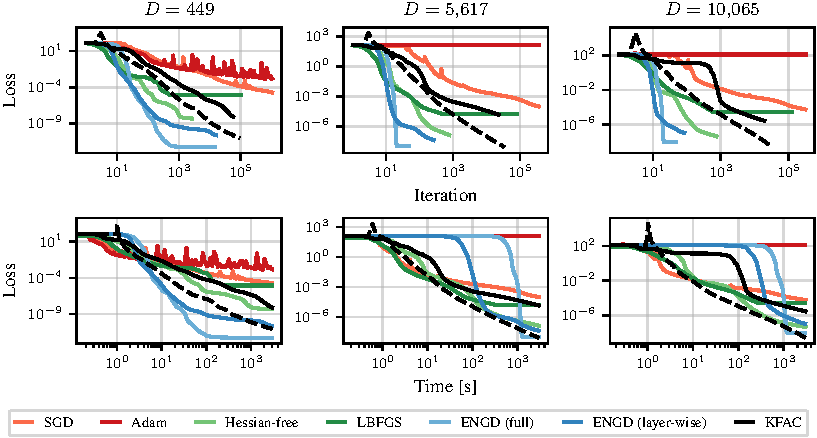
\includegraphics{../kfac_pinns_exp/exp18_groupplot_poisson5d/loss.pdf}
  \caption{Scaling behaviour of different optimizers for learning the solution of a 5d-Poisson equation w.r.t.
    neural network size under a given time budget of $3\cdot 10^3\,\text{s}$ on an RTX 6000 GPU.}
  \label{fig:pedagogical-example}
\end{figure}

\subsection{Setup}
We implement KFAC, KFAC*, as well as the diagonal, block-diagonal, and full-Gramian ENGD in PyTorch~\citep{paszke2019pytorch}.
As a matrix-free version of ENGD, we use the HessianFree optimizer~\citep{?} which uses truncated CG with exact Gramian-vector products to pre-condition the gradient.
We chose this because there is a fully-featured implementation from~\citet{tatzel2022late} which offers many additional heuristics such as adaptive damping, CG backtracking, and backtracking line search, which allows this algorithm to be operated with very little hyperparameter searching.
We also use SGD with a tuned learning rate and momentum, as well as Adam with a tuned learning rate.
Experiments are run on a compute cluster with RTX 6000 GPUs (24\,GiB RAM).

\paragraph{Experimental setup}
\begin{itemize}
\item hyper-parameter search
\end{itemize}


\subsection{Pedagogical example: 2D Poisson and 1D Heat}

We consider the two low-dimensional PDEs used to demonstrate the efficacy of energy natural gradients by~\cite{muller2023achieving}
as we can use it as a baseline here for its KFAC-approximation. 
The problems are given by the two-dimensional Poisson equation 
\begin{align}
    -\Delta u(x,y) = ? \\ 
    asdf
\end{align}
as well as the one-dimensional heat equation 
\begin{align}
\partial_t u(x,t) - \kappa \Delta u(x,t). 
\end{align}
Here, we choose the heat-conductivity $\kappa = \frac14$ in our experiments. 

We evaluate the performance of various optimizers... for different network architectures with $4$ hidden layers of different widths and the hyperbolic tangent $\tanh$ as an activation function. 

\begin{itemize}
    \item write down equations 
    \item Netzwerkarchitekturen
\end{itemize}


\subsection{A high dimensional Poisson equation}

\begin{itemize}
\item 100D from deep Ritz paper~\citep{yu2018deep}, i.e.,
  \begin{align*}
    -\Delta u(x) & = -200 \quad \text{for } x\in [0,1]^{100} \\
    u(x) & = \lVert x \rVert_2^2 \quad \text{for } x\in \partial[0,1]^{100}
  \end{align*}
  where the solution is given by $u^\star(x) = \lVert x \rVert_2^2$
\item around $10^5$ to $10^6$ parameters
\item no ENGD, ENGD matrix-free?, only KFACs, L-BFGS, HF, and first-order methods
\end{itemize}


\subsection{Heat equation}

\begin{itemize}
\item again 100D
\item sum of cosinuts with exponential trash in time? I.e.,
  time-space domain $[0,1]\times[0,1]^{100}$ %and
  % \begin{align*}
  %   \partial_t u(t,x)-\Delta_x u(t,x) & = 0 \quad \text{for } x\in [0,1]^{100} \\
      %       u(0,x) & = \sum_{i=1}^{100} \sin(\pi x_i) \quad \text{for }
  %   x\in [0,1]^{100}
  %   \\
  %   u(t,x) & = 0 \quad \text{for } t\in[0,1], x\in\partial[0,1]^{100}
  % \end{align*}
  % \item an alternative would be
  \todo{rhs not equal zero I think, double check before implementing}
  \begin{align*}
    \partial_t u(t,x)-\Delta_x u(t,x) & = 0 \quad \text{for } x\in [0,1]^{100} \\
    u(0,x) & = \sum_{i=1}^{100} \sin(\pi x_i) \quad \text{for }
             x\in [0,1]^{100}
    \\
    u(t,x) & = e^{-\pi^2 t}\sum_{i=1}^{100} \sin(\pi x_i) \quad \text{for } t\in[0,1], x\in\partial[0,1]^{100}
  \end{align*}
  for which the solution should be given by
  \begin{align*}
    u^\star(t,x) = e^{-\pi^2 t} \sum_{i=1}^{100} \sin(\pi x_i)?
  \end{align*}
  % we can also scale in time because $e^{-4\pi^2}\approx e^{-40}$
\item around $10^5-10^6$ parameters
\end{itemize}

\subsection{Discussion}

Hessian free vs KFAC (KFAC plays nicer with stochasticity?!)

\subsection{Limitations and Future Work}

\paragraph{Studying further KFAC heuristics} The original KFAC optimizer introduces many additional techniques to improve performance and stability, e.g.\,adaptive damping and heuristics for splitting up the damping onto the different Kronecker factors.
Our algorithms borrow components, but we did not explore all bells and whistles.
We believe they can help to either reduce the number of hyper-parameters that need to be tuned, or improve performance.
We use an independent Kronecker product for each of the losses and dit not look into further condensing this representation into a single Kronecker product.
Doing so would allow to further reduce memory cost for storing the pre-conditioner, as well as computational cost to invert it.
We did not play around with updating the KFAC matrices or inverting the pre-conditioner less frequently.
We did not try lower precision than float64 because this is the standard setup for PINNs (??).

\paragraph{Performance improvements} The generalized eigenvalue that we currently need to solve to invert the Kronecker sum is currently computed through SciPy as there is no PyTorch API for doing so. This has the downside that we need to sync the Kronecker factors with CPU each time we want to invert the curvature approximation. Our results could be further improved by using a fully GPU-compatible implementation.
As pointed out in \citep{martens2015optimizing}, the requested Gramian projections can be computed at the cost of two forward passes; however, we are currently using a non-specialized implementation which does not take into account the Gramian's matrix square root factorization.
One could also merge the backward pass for each Gramian with that of its loss into a single backward traversal rather than two sequential ones, e.g.\,as done by~\cite{dangel2020backpack}.
However, then one needs to manually implement the additional backpropagation (through both the normal forward pass, but also through the forward Laplacian pass).

\paragraph{Future work}
Inverse-free KFAC update~\citep{lin2023simplifying} and structured Kronecker factors~\citep{lin2023structured}.

\begin{comment}
  We want to show the following things:
  \begin{itemize}
  \item We can safely discard the Gramian's off-diagonal blocks without harming
    training performance. This reduces the Gramian's size, but still imposes
    strong constraints on scalability.

  \item Our proposed Kronecker approximation works roughly as well as the
    full/block diagonal Gramian, while being much cheaper to compute, store, and
    invert.

  \item Thanks to the Kronecker approximation of the Gramian, we can scale to larger neural networks where the other methods either do not work (storing the Gramian is prohibitively expensive) or become quite slow (matrix-free linear system solve via Gramian-vector products).
  \end{itemize}

  Todos:
  \begin{itemize}
  \item concrete example ground truth: 2d Poisson on unit square with sine target
  \end{itemize}

  Ideas:
  \begin{itemize}
  \item try out different approximations
    \begin{itemize}
    \item Ground truth
    \item Block diagonal exact
    \item Diagonal
    \item Block diagonal with different approximations
    \end{itemize}
  \end{itemize}
\end{comment}

%%% Local Variables:
%%% mode: latex
%%% TeX-master: "../main"
%%% End:
